\documentclass[a4paper, 11pt, twoside]{article}

\usepackage[utf8]{inputenc}
\usepackage{lmodern}
\usepackage[T1]{fontenc}
\usepackage[francais]{babel}
\usepackage{draftwatermark} %Gestion du filigranne
\usepackage{graphicx} 
\usepackage[dvipsnames]{xcolor} %Personnalisation des couleurs
\usepackage{tikz}
\usepackage{enumitem} %Personnalisation des listes à puces
\usepackage[normalem]{ulem} %Barrer du texte
\usepackage{bigstrut} %tableau Excel -> LaTeX
\usepackage{verbatim}
\usepackage{braket}
\usepackage{fancybox}
\usepackage{etoolbox}
\usepackage{tkz-tab}
\usepackage{microtype}
\usepackage{pgfplots}
\usepackage[hypertexnames=false]{hyperref}
\hypersetup{colorlinks = true, linkcolor = black, urlcolor = black, citecolor = black}
%Gestion du filigrane
\SetWatermarkLightness{0.75}
\SetWatermarkAngle{45}
\SetWatermarkScale{2}
\SetWatermarkFontSize{2cm}

\usepackage{amsmath}
\usepackage{amsfonts}
\usepackage{amssymb}
\usepackage{dsfont}
\usepackage{esint}
\usepackage{fancyhdr}

%En tête et pied de page
\pagestyle{fancy}
\lhead[]{}
\chead[]{}
\rhead[]{}
\lfoot[\thepage]{}
\cfoot[]{}
\rfoot[]{\thepage}

\renewcommand{\headrulewidth}{0mm}
\renewcommand{\footrulewidth}{0.0 mm}
\numberwithin{equation}{subsection}
\renewcommand{\theequation}{\Roman{section} . \arabic{subsection}\arabic{equation}}
% Format des sections
\csname @addtoreset\endcsname{section}{part}
\renewcommand\thepart{\Roman{part})}
\renewcommand\thesection{\Roman{section}.}
\renewcommand\thesubsection{\arabic{subsection})}
\renewcommand\thesubsubsection{\alph{subsubsection}.}

%Gestion des listes à puces
\setitemize[1]{label = $-$}
\setitemize[0]{label = $\hookrightarrow$}

\newbool{Couleur}
\newcommand{\couleur}[1]{\ifbool{Couleur}{\color{#1}}{}}

%----------------------------------------------------------------------------
%Théorème : Commande : \Thm[Nom éventuel]{} (couleur : marron)
%Exercices : Environnement : {Exo}
%Démonstration : Environnement : {Demo} (couleur : violet)
%Définition : Commande : \Def[Nom éventuel]{Nb de defintion(s)}{} (coul :vert)
%Propriétés : Commande : \Pro[Nom éventuel]{Nb de propriété(s)}{} (coul :red)
%Systèmes : Environnement : {Syst}
%Cadre : Environnement : {Cadre}
%Solution : Environnement : {Solution} (Peut être enlever avec la commande \exclure - couleur : bleu)
					%---------------------------------%
\setlength {\shadowsize}{2pt}
%Environnement pour les exercices
\newcounter{exo}
\newenvironment{Exo}{\stepcounter{exo} \textbf{Exercice \theexo \medbreak} 
\renewcommand{\theequation}{\arabic{equation}}
\setcounter{equation}{0}}{}

%Commande pour les théorèmes
\newcounter{th}\newcommand{\Thm}[2][]{\couleur{brown}\vspace{3ex}\boxput*(-0.4,1){\setlength{\fboxsep}{0pt}\colorbox{white}{\setlength{\fboxsep}{1ex}\Ovalbox{{\textsc{\ifstrequal{#1}{}{Théorème \stepcounter{th} \theth \phantom{}}{Théorème \stepcounter{th} \theth \phantom{} : #1}}}}}}{\setlength{\fboxsep}{7mm}\doublebox{\noindent \begin{minipage}{0.95\linewidth}\vspace{1ex}#2\end{minipage}}}\vspace{1ex}\couleur{black}}

%Environnement pour les Démonstration :
\newenvironment{Demo}{\couleur{RoyalPurple} \begin{itshape}Démonstration :\\}{\begin{flushright} Qed \end{flushright} \end{itshape}\couleur{black}}

%Commande pour les définitions
\newcommand{\Def}[3][]{\couleur{Green}\vspace{3ex}\boxput*(-0.4,1){\setlength{\fboxsep}{0pt}\colorbox{white}{\setlength{\fboxsep}{1ex}\Ovalbox{{\textbf{\ifnumequal{#2}{1}{\ifstrequal{#1}{}{Définition}{Définition : #1}}{\ifstrequal{#1}{}{Définitions}{Définitions : #1}}}}}}}{\setlength{\fboxsep}{7mm}\fbox{\noindent \begin{minipage}{0.95\linewidth}\vspace{1ex}#3\end{minipage}}}\couleur{black}\vspace{1ex}}

%Commande pour les propriétés
\newcommand{\Pro}[3][]{\couleur{red}\vspace{3ex}\boxput*(-0.4,1){\setlength{\fboxsep}{0pt}\colorbox{white}{\setlength{\fboxsep}{1ex}\Ovalbox{{\textbf{\ifnumequal{#2}{1}{\ifstrequal{#1}{}{Propriété}{Propriété : #1}}{\ifstrequal{#1}{}{Propriétés}{Propriétés : #1}}}}}}}{\setlength{\fboxsep}{7mm}\shadowbox{\noindent \begin{minipage}{0.95\linewidth}\vspace{1ex}#3\end{minipage}}}\couleur{black}\vspace{1ex}}

%Environnement pour les systèmes
\newenvironment{Syst}{\begin{equation} \left\{ \begin{array}{c @{\hspace{0.2cm} = \hspace{0.2cm} } c}}{\end{array} \right. \end{equation}}

%Envrionnement pour la solution des exercices
\newenvironment{Solution}{\couleur{blue}\begin{flushleft}\begin{tikzpicture}[overlay]\draw(0,0) arc(90:180:1);\draw(0,0)--(0.5,0) node[right]{\underline{\texttt{\textbf{Correction :}}}};\draw(-1,-1)--(-1,-1.5);\end{tikzpicture} \end{flushleft}}{\begin{flushright}\begin{tikzpicture}[overlay]\draw(0,0) arc (270:360:1);\draw(0,0)--(-0.5,0);\draw(1,1)-- (1,1.5);\end{tikzpicture}\end{flushright}\couleur{black} \vspace{1 cm}}
\newcommand{\exclure}[1]{\renewenvironment{#1}{\begingroup\comment}{\endcomment\endgroup\ignorespaces}}

%Environnement d'encadrement du texte
\setlength{\fboxsep}{5mm}
\newsavebox{\fmbox}
\newenvironment{Cadre}
     {\begin{lrbox}{\fmbox}\begin{minipage}{0.9\textwidth}}
     {\end{minipage}\end{lrbox}\fbox{\usebox{\fmbox}}\\}

\newcommand{\ssi}{\textrm{ si et seulement si }}
\newcommand{\defi}{\underset{def}{\equiv}}
\renewcommand{\arraystretch}{1.8}
\newcommand{\rem}[1]{\textit{\underline{Remarque :} #1}}



%Code pour le tracé d'une fonction
	\iffalse
	\begin{tikzpicture}
		\begin{axis}[
		title  = ...,
		xlabel = ...,
		ylabel = ...,
		domain = :]
		\addplot[blue]{...};
		\end{axis}
	\end{tikzpicture}
	\fi

% -----------------------------------------------------------------------

\title{Module Pile à hydrogène \\ Déroulé V4}
\author{}
\date{}
\SetWatermarkText{\textsc{}} %Texte du filigrane

%OPTIONS DU DOCUMENT : (solution (avec ou sans); couleur ou N&B)
%\exclure{Solution} %Retire les environnements solution
\booltrue{Couleur} %Texte en couleur
%\boolfalse{Couleur} %Texte en N&B

\begin{document}
	\renewcommand{\contentsname}{Sommaire}
	
% -----------------------------------------------------------------------	
	\maketitle
	\pagestyle{fancy}
	
	\section*{Introduction}
	
	Le module présenté dans ce document concerne uniquement la pile à hydrogène. Ce module fera partie d'un atelier plus global sur l'énergie à destination de collégiens.
	
	Ainsi, cette partie sur la pile à hydrogène sera introduite par d'autres activités qui aborderont probablement la distinction entre les productions mécanique, chimique et photovoltaïque.

	\section{Descriptif du système : document animateur}
	
	\subsection{Présentation du fonctionnement (circuit complet)}
		
		Les piles à hydrogène permettent à partir de dihydrogène et de dioxygène de produire de l'électricité. \footnote{Certaines piles à combustible fonctionnent à l'aide de combustible différent (gaz ou liquide), c'est le cas par exemple de la pile à méthanol.}
	
	Le dioxygène présent dans l'air peut-être utilisé pour faire fonctionner ces piles. Cependant, nous étudierons plutôt \emph{l'électrolyse de l'eau} pour former du dihydrogène et du dioxygène. Ce phénomène nécessite un apport extérieur d'énergie car la réaction n'est pas thermodynamiquement favorisée.
	
	Ainsi, le circuit complet se décompose en trois étapes principales :
	\begin{itemize}
		\item Apport d'énergie
		\item Électrolyse de l'eau pour former du $O_2$ et du $H_2$.
		\item Fonctionnement de la pile (cf équation (\ref{pile})) avec production d'électricité
	\end{itemize}
	
	\subsection{Apport d'énergie}
	
	Pour avoir lieu, l'électrolyse de l'eau nécessite un apport d'énergie extérieure. 
	
	Celle-ci peut prendre différentes formes en général : énergie nucléaire, énergie solaire, énergie éolienne ou énergie hydraulique.
	
	Expérimentalement, on peut utiliser : une alimentation\footnote{En faisant attention aux consignes constructeurs concernant l'électrolyseur}, des maquettes de panneaux solaires, des maquettes d'éoliennes et une dynamo pour faire prendre conscience de l'apport d'énergie.
	
	Les différents moyens d'apporter l'énergie ont tous pour conséquence de fabriquer les deux gaz attendus plus ou moins rapidement (en fonction des maquettes).
	
	\subsection{Électrolyse de l'eau}
	\subsubsection{Présentation théorique}
	L'électrolyse de l'eau permet de former du $H_2$ et du $O_2$ à partir d'eau distillée selon les demi équations d'oxydoréduction suivantes (pour une pile à membrane échangeuse de protons) \cite[Page 26]{These}:
	
	\begin{equation}
		2H_2O \rightarrow O_2 + 4H^+ + 4e^- \textrm{ à l'anode (oxydation)}
	\end{equation}
	\begin{equation}
		2H^+ + 2e^- \rightarrow H_2 \textrm{ à la cathode (réduction)}
	\end{equation}
	
	L'équation totale de la réaction est donc :
	\begin{equation}
		2H_2O \rightarrow O_2 + 2H_2
	\end{equation}
	
	Une représentation possible d'une cellule d'électrolyse est la suivante:
	\begin{figure}[!h]
		\begin{center}
			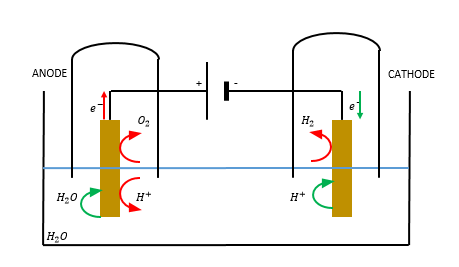
\includegraphics[scale=1]{Electrolyse}
			\caption{Schéma de fonctionnement d'un électrolyseur}
			\label{Electrolyse}
		\end{center}
	\end{figure}
	
	
	\newpage
	
	Sur la Figure \ref{Electrolyse}, les flèches rouges représentent des produits alors que les flèches vertes représentent les réactifs.
	
	Les cloches situées au dessus de l'anode et de la cathode permettent de récupérer les gaz dans deux récipients distincts : du dioxygène au niveau du tube situé à l'anode et du dihydrogène au niveau du tube situé à la cathode.
	
	\rem{La st\oe chiométrie des réactions n'est pas mise en évidence sur le schéma.}
	
	\subsubsection{Schéma d'un électrolyseur}
	
	Les électrolyseurs utilisés lors des manipulations sont plus compacts et on ne voit pas les deux électrodes séparées. Les cellules d'électrolyse utilisées ressemblent plutôt à cela :
	
	\begin{figure}[!h]
		\begin{center}
			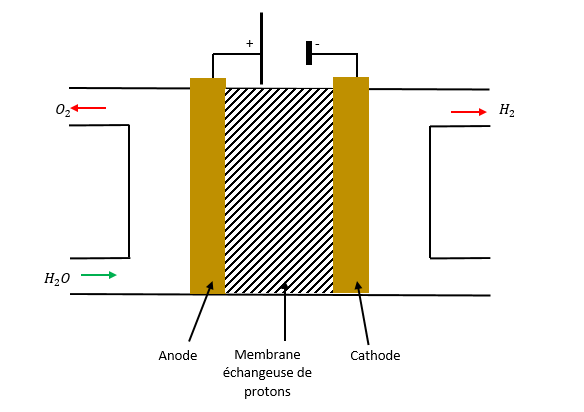
\includegraphics[scale=0.8]{Schemfoncelectrolyse}
			\caption{Schéma de l'électrolyseur utilisé}
		\end{center}
	\end{figure}
	
	Les électrons circulent dans le circuit électrique et dans les électrodes alors que les ions $H^+$ circulent dans la membrane échangeuse de protons.
	
	Les électrodes sont fabriquées à partir de métaux précieux (platine,...) qui servent de catalyseurs aux réactions qui ont lieu à l'anode et à la cathode.
	
	Pour utiliser correctement un électrolyseur, il faut suivre les instructions données par le constructeur. 
	
	\subsection{Fonctionnement de la pile}
	
	La pile fonctionne suivant les équations d'oxydoréduction suivantes (pour une pile à membrane échangeuse de protons) :
	\begin{equation}\label{demi1}
		H_2 \rightarrow 2H^+ + 2e^- \textrm{ à l'anode (oxydation)}
	\end{equation}
	
	\begin{equation}\label{demi2}
		O_2 + 4H^+ + 4e^- \rightarrow 2H_2O	\textrm{ à la cathode (réduction)}
	\end{equation}
	
	L'équation de réaction globale est donc la suivante :
	\begin{equation}\label{pile}
		2H_2 + O_2 \rightarrow 2H_2O
	\end{equation}
	
	\rem{Par rapport à l'électrolyseur, les électrodes (anode et cathode) sont "échangées". Il faut savoir que l'oxydation se produit \emph{toujours} à l'anode. Ainsi, on détermine sans erreur la nature des électrodes. De plus, les électrons sortent \emph{toujours} de l'anode ce qui permet de déterminer le sens du courant.}
	
	\begin{figure}[!h]
		\begin{center}
			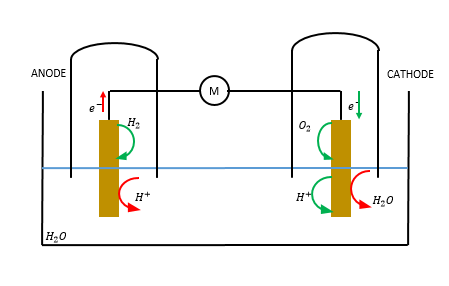
\includegraphics[scale=1]{Schempile}
			\caption{Schéma de fonctionnement d'une pile à hydrogène}
		\end{center}
	\end{figure}
	
	\rem{La st\oe chiométrie des réactions n'est pas mise en évidence sur le schéma.}
	
	\vspace{5 cm}
	Les piles disponibles sur les tables ressemblent plutôt au schéma suivant :
	
	\begin{figure}[!h]
		\begin{center}
			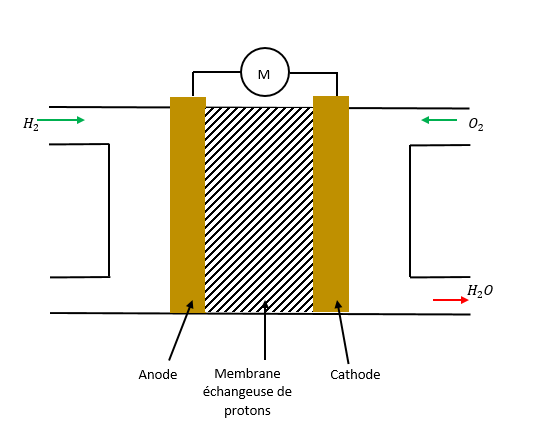
\includegraphics[scale=1]{Schemfoncpile}
			\caption{Schéma pile utilisée}
		\end{center}
	\end{figure}
	
	On retrouve dans un système compact l'anode du côté $H_2$ et la cathode du côté $O_2$. 
	
	La membrane échangeuse de protons laisse le passage libre aux ions $H^+$ mais bloque le passage des électrons qui passent dans le circuit, d'où la production d'électricité.
	
	\rem{La membrane joue le rôle d'une solution électrolytique assurant la neutralité de toutes les espèces en présence. De plus, elle permet de séparer les deux gaz.}
	
	Certains modèles de pile à hydrogènes sont réversibles. C'est-à-dire que le même système joue le rôle de pile et d'électrolyseur.
	
	\subsection{Les difficultés expérimentales.}
	
		\subsubsection{Les difficultés}
	Lors des essais réalisés sur différents modèles d'électrolyseur et de pile à hydrogène (maquettes pédagogiques), nous avons soulevé un certain nombre de difficultés expérimentales lorsque l'on branche une pile à un consommateur (LED, moteur, etc...).

	Pour les montages dans lesquels le consommateur ne nécessite pas une trop grande puissance, la pile permet la mise en marche du consommateur. Cependant, il faut attendre un long moment pour voir la diminution des niveaux de gaz.
	
	À contrario, dans les montages où le consommateur nécessite une forte puissance, la pile ne suffise pas toujours à le mettre en fonctionnement et on ne voit pas du tout la consommation de gaz. 
	
	Certains montages, à mi-chemin entre les deux précédents, permettent le fonctionnement pendant un court laps de temps du consommateur sans visualisation de la consommation de gaz.
	
	Dans tous les cas, on ne voit jamais que la pile s'arrête à cause du manque de l'un des deux gaz. En effet, lorsque le consommateur s'arrête, il reste du gaz. L'arrêt du consommateur et la non consommation du gaz peut s'expliquer de deux façons différentes. Soit le gaz restant n'est plus pur et ne permet à la pile de fonctionner correctement, soit il n'y a plus suffisamment de pression pour que les gaz atteignent la pile permettant la mise en marche du consommateur.

	L'humidification de la membrane interne de la pile empêche la pile de fonctionner. Il faut parfois sécher ou humidifier à nouveau celle-ci. Dans tous les cas, les constructeurs déconseillent fortement le démontage des piles (cela dépend des piles). 
		
	\subsubsection{Quelques solutions}
	Pour résoudre certaines de ces difficultés, nous avons trouvé quatre solutions qui peuvent fonctionner. 
	
	Dans un premier temps, il peut être utile d'effectuer une purge soit du côté dihydrogène ($H_2$), soit du côté dioxygène ($O_2$). En effet, il est possible que les gaz contenus dans les réservoirs ne soient pas purs et il est donc nécessaire d'évacuer l'air au niveau de la pile. 
	
	\rem{Les purges doivent être faites par l'animateur car il faut faire attention à ne pas vider tous les gaz contenus dans les réservoirs.}
	
	Il est également possible de mettre en court-circuit la pile afin de supprimer les potentiels excédents de charge. 
	
	Enfin, il faut être attentif à la hauteur d'eau située au-dessus des gaz. En effet celle-ci est directement liée à la pression des gaz ; ainsi une hauteur d'eau insuffisante est équivalente à un manque de pression ce qui entraine l'arrêt du fonctionnement de la pile.
	
	Pour l'instant, aucune solution concernant l'humidification de la membrane n'a été trouvé. \footnote{Certains constructeurs insistent sur l'humidification de la membrane dans les règles de mise en marche de ma pile.}
	
	\subsubsection{Bilan}
	
	Même s'il existe des solutions afin d'assurer le bon fonctionnement de la pile, il n'existe pas vraiment de protocole afin de savoir d'où vient réellement le problème. Ainsi, il est nécessaire d'essayer toutes les solutions afin de relancer la pile.
	
	Toutes ces difficultés techniques nécessitant une attention particulière de l'animateur, il est plus adapté d'utiliser \emph{une seule pile par îlot}.
	
	Nous n'avons pas rencontré de problème particulier concernant la partie électrolyse. Ainsi, il est envisageable d'utiliser \emph{un électrolyseur par binôme} afin de fabriquer un maximum de gaz, utilisable par la suite par l'unique pile de l'îlot. L'animateur sera tout de même attentif à ce que les élèves ne produisent pas trop de gaz (bulles au niveau du réservoir $H_2$) afin qu'il y ait le moins de $H_2$ dans la pièce (inflammable).
	
	\section{Descriptif du contenu pédagogique de mode d'emploi en cours d'atelier}
		\subsection{Électrolyse de l'eau}
		
		\subsubsection{Compréhension du fonctionnement}
		
		\paragraph{Réaction chimique\\}
		
		On donne par binôme un modèle moléculaire représentant l'eau.
				
		L'animateur de son côté montre un modèle de la molécule de dihydrogène ($H_2$) et un modèle de la molécule de dioxygène ($O_2$) (deux gaz).
		
		Il demande aux élèves de modifier la molécule d'eau afin de former ces deux molécules.
		
		Les élèves constatent qu'il y a un problème. Il manque un oxygène (boule rouge) pour former le dioxygène ($O_2$). Ils en demandent une mais l'animateur ne peut donner que des modèles représentant de l'eau. Ainsi, ils remarquent qu'il leur faut deux molécules de $H_2O$ et qu'ils peuvent ainsi faire une molécule de $O_2$ et deux de $H_2$. 
		
		Les élèves ont ainsi mis en évidence la réaction chimique suivante :
		\begin{equation} \label{rea}
			2H_2O \rightarrow 2H_2 + O_2
		\end{equation}
		\newpage
		
		\rem{La notion de réaction chimique n'est abordée que en 3$^{e}$.}
		
		\rem{Pour les $3^{e}$, il peut être intéressant de revenir sur les notions de molécules et d'atomes. Chaque molécule étant constituée de plusieurs atomes ayant chacun leur caractéristique (taille, masse, couleur dans les modèles, etc...) On ne parle pas de la charge. Il s'agit d'un bonus "explicatif".}
		
		\paragraph{L'apport d'énergie électrique\\}
		
		Il est important que les élèves comprennent que l'eau ne se transforme pas naturellement en dihydrogène et en dioxygène. La réaction (\ref{rea}) nécessite un apport d'énergie extérieur.
		
		On peut mettre en évidence la nécessité de cet apport en utilisant la dynamo. L'utilisation de la dynamo souligne bien l'effort nécessaire à la production des gaz.
		
		L'animateur doit expliquer que les molécules sont fragilisées par le mouvement des électrons apportées par l'alimentation extérieure. Ainsi ces électrons "séparent" les molécules qui se regroupent pour former d'autres molécules plus stables.
		
		
		\rem{Si la notion électricité = déplacement d'électrons a été vue précédemment, il peut être utile de préciser que la réaction (\ref{rea}) a lieu car il y a un échange (déplacement) d'électrons (oxydoréduction).}
		
	\subsubsection{L'électrolyse}
	
	L'animateur peut utiliser une alimentation électrique externe pour accélérer la production de gaz. 
	
	\rem{L'alimentation électrique doit absolument être choisie en fonction de la cellule d'électrolyse choisie (à voir sur la notice constructeur).}
	
	\rem{Il faut faire attention à la polarité des branchements.}
	
	On remarque que les deux gaz se placent dans deux tubes différents (l'un est noté $H_2$ et l'autre $O_2$). On explique aux élèves qu'il existe un système chimique qui permet de séparer ces deux gaz. (Ce système est en fait la membrane échangeuse de protons).
	
	Les élèves devraient remarquer qu'il y a environ deux fois plus dihydrogène que de dioxygène formé pendant la production des deux gaz. L'animateur doit les amener à faire le lien avec la st\oe chiométrie de la réaction $2H_2O \rightarrow 2H_2 + O_2$. Le facteur n'est pas totalement vérifié à cause des niveaux initiaux de gaz, des potentielles fuites du côté du dihydrogène.
	
	
	\rem{La st\oe chiométrie est vérifiée tout au long de la production du gaz lors de l'électrolyse. Ainsi, si chaque binôme a un électrolyseur, les élèves pourront mieux suivre l'évolution de la production des deux gaz et constater qu'il y a deux fois plus de $H_2$ que de $O_2$. (Deux électrolyseurs par tables est aussi envisageable).}
	
	\subsubsection{Quelles sources d'énergie externe ?}
	
	La production de dihydrogène (si elle se fait par électrolyse de l'eau) nécessite un apport extérieur d'énergie. \\
	
	\textit{Discours général :}
	
	Pour que la pile soit vraiment une source d'énergie propre, il faut que le dihydrogène soit également produit proprement. Pour ce faire, il peut être envisageable d'utiliser les surplus d'énergies renouvelables telles que le solaire, l'éolien ou l'hydraulique. Actuellement, ceci est peu fait car il est préférable de consommer directement l'énergie produite. Cependant, le navire \emph{Hydrogen Challenger} utilise l'électricité provenant d'une éolienne afin de produire de l'hydrogène. \footnote{Manque de référence sur le système de conversion, mais c'est l'idée que l'on veut faire passer : utiliser les surplus d'énergies renouvelables pour fabriquer de l'hydrogène.}
	
	De façon plus générale, l'hydrogène est fabriqué à partir de méthodes chimiques telles que :
	\begin{itemize}
		\item La réduction de la vapeur d'eau :
		$$
			CH_4 + H_2O \rightarrow CO + 3H_2
		$$
		
		Cette méthode est polluante car on constate la formation de monoxyde de carbone ($CO$) gaz dangereux pour l'homme et pour l'environnement. Cependant, ce gaz peut être réutilisé donnant lieu à la réaction suivante :
		$$
			CO + H_2O \rightarrow CO_2 + H_2
		$$
		
		Méthode également polluante car il y a formation d'un gaz à effet de serre bien connu, le dioxyde de carbone.
		
		\item Méthodes biologiques
		\item Production thermochimique à haute température
		\item etc...
	\end{itemize}
	
	La plupart de ces méthodes sont plus utilisées que l'électrolyse car elles ont un meilleur rendement mais sont plus polluante que l'électrolyse de l'eau (lorsque celle-ci est faite à partir d'énergie renouvelable).
	
	D'un point de vue du matériel expérimental et pédagogique, des maquettes solaires, éoliens et hydrauliques peuvent être utilisées mais il faut faire attention à ne pas tirer de conclusions hâtives et à ne pas généraliser les résultats obtenus à l'aide des maquettes.
	
	\newpage
	\subsubsection{Objectifs de la partie}
	
	Les élèves doivent avoir compris que :
	\begin{itemize}
		\item L'électrolyse permet la production de gaz (dioxygène et dihydrogène),
		\item La réaction (\ref{rea}) nécessite un apport d'énergie extérieure,
		\item (Notion de réaction chimique) 
	\end{itemize}
	
	\subsection{Fonctionnement de la pile}
	
	\rem{Pré-requis : Mouvement d'électrons $\Leftrightarrow$ électricité}
	
	\subsubsection{Introduction}
	
	Questionnement élèves : Quel est l'intérêt d'avoir fabriquer ces deux gaz ?
	
	La réaction (\ref{rea}) est réversible et produit de l'eau et de l'électricité.
	
	Pour faire fonctionner la pile, on branche les deux arrivées de gaz sur le dispositif en suivant les consignes du constructeur et on branche en sortie un consommateur (moteur, LED, ...).\footnote{Voir figure 4.}	
	
	On a stocke l'énergie sous forme de gaz.
	
	\subsubsection{Manipulations envisageables}
	
	Des circuits simples utilisant la pile à hydrogène comme source d'électricité. 
	
	\rem{S'il y a besoin de faire des rappels sur les différents types de circuit pour la suite de l'atelier, il est possible d'utiliser ce type de pile plutôt qu'une alimentation classique.}
	
	\subsection{Bilan}
	
	Faire faire un bilan aux élèves de ce qu'ils ont vu :
	\begin{itemize}	
	\item Comment on forme les deux gaz (à partir de l'électrolyse de l'eau).
	
	\item Leur faire compléter une chaine d'énergie (avec le stockage dans le milieu sous forme d'énergie chimique).
	\end{itemize}
	
	\newpage
	\section{Applications et avantages de la pile à hydrogène}
	
	\begin{itemize}
		\item Système mobile :
			\begin{itemize}
				\item Automobile :
				
				Toyota a développé un modèle de voiture utilisant la pile à hydrogène : la toyota Miraï. \cite{Toyota}
				
				Fonctionne avec une pile $H_2$/air. Le dihydrogène est stocké dans deux réservoirs en fibre de carbone.
				
				Elle est dotée d'une unité de contrôle ainsi que d'une batterie pour gérer la production et le stockage d'électricité.
				
				Choix de l'hydrogène : disponible partout (eau, plante ...)
				
				En plus d'être un système embarqué, la production du dihydrogène peut-être propre (gazéification, reformage du méthane ou électrolyse à partir d'énergie renouvelable).
				
				\begin{figure}[!h]
					\begin{center}
						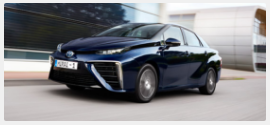
\includegraphics[scale=0.7]{Toyota}
						\caption{Photo d'une Toyota Miraï}
					\end{center}
				\end{figure}
			
			\item Certaines collectivités investissent dans l'énergie hydrogène pour leurs flottes de véhicules d'entretien de voirie ou des espaces verts.
			\item Spatial \cite{Spatial}:
				Le vaisseau Appolo utilise une pile à hydrogène de type AFC (avec de l'hydrogène et de l'oxygène liquide).
			
		\end{itemize}
		
		\item Stationnaire dans certain domicile : pile à combustible (gaz naturel, pas du dihydrogène). Viessman et Vaillant proposent des chaudières à micro-cogénération à pile à combustible qui à partir de gaz naturel produisent de l'électricité, du chauffage et rejettent seulement de l'eau.
		
		\item C'est un système propre à partir du moment où l'obtention de l'hydrogène se fait proprement en utilisant un surplus de production ou des énergies renouvelables. \footnote{Le craquage du pétrole permet d'obtenir de façon pas écologique du dihydrogène mais est utilisé dans certains pays.}
	\end{itemize}
	
	Des recherches sont en cours sur les piles à hydrogène afin de les développer et de pouvoir les utiliser à plus grande échelle.
	
	Pour l'instant le coût de ces piles est élevé et cela est notamment dû au prix des électrodes (en platine ou autres métaux rares) qui servent de catalyseur. Au sein du projet MOMENTOM porté par l'Université Paris-Saclay, un groupe de recherche travaille sur une catalyse organo-métallique afin de faire diminuer le coût de production. 
	
	D'autres recherches portent sur :
	\begin{itemize}
		\item Une amélioration des rendements de ce type de pile,
		\item Un allongement de l'espérance de vie de ces piles,
		\item Les matériaux utilisés,
		\item Le stockage des gaz,
		\item etc... 
	\end{itemize}
	
	\bibliographystyle{apalike-fr}
	\bibliography{Biblio}
\end{document}
